%%%%%%%%%%%%%%%%%%%%%%%%%%%%%%%%%%%%%%%%%%%%%%%%%%%%%%%%%%%%%%%%%%%%%%%%
% Plantilla TFG/TFM
% Universidad de A Coruña. Facultad de Informática
% Realizado por: Welton Vieira dos Santos
% Modificado: Welton Vieira dos Santos
% Contacto: welton.dossantos@udc.es
%%%%%%%%%%%%%%%%%%%%%%%%%%%%%%%%%%%%%%%%%%%%%%%%%%%%%%%%%%%%%%%%%%%%%%%%


\chapter{Análisis de Viabilidad: Modelado de la Organización.}

\section{Formulario OM-1: Contexto Organizacional, problemas y soluciones.}
Identificación de los problemas y oportunidades orientadas al conocimiento de la organización, como se muestra en la Tabla \ref{tab:OM1}.


\begin{table}[H]
\scriptsize
\begin{tabularx}{\textwidth}{|l|X|} \hline
\textbf{Modelo de Organización} & \textbf{Formulario OM-1: Problemas y Posibilidades de Mejora} \\ \hline\hline

\textsc{Problemas y Oportunidades} & Invertir o especular con activos financieros en bolsa de valores es una labor bastante compleja, ya que si una persona no tiene el conocimiento suficiente y adecuado puede ser un auténtico ``desastre''. Con ese panorama, se presenta una oportunidad para desarrollar sistemas que sean capaces de hacer esa labor con el menor error posible y con ganancias muy superior a media de operaciones hechas actualmente en el mercado financiero. Además de acercar esa práctica de inversión a particulares (conocidos como inversores minoritarios), que generalmente no tiene mucho capital para hacer inversiones mas seguras.\\ \hline
\textsc{Contexto Organizacional} & 
\begin{enumerate}
  \item La Misión, visión y objetivos de la organización son:  
  \begin{enumerate}
    \item \textbf{Misión:} Una pequeña empresa (Startup) de desarrollo de aplicaciones inteligentes relacionadas con el mercado financiero.
    \item \textbf{Visión:} Dando continuidad de un sistema inteligente desarrollado anteriormente, donde el sistema sólo lidiaba con mercados de acciones y ahora funcionará con los mercados de divisas (Forex).
    \item \textbf{Objetivos:} Seguir creciendo como empresa desarrolladora y seguir expandiendo las ventas de nuestras soluciones inteligentes para que en el futuro se pueda comercializar de forma globalizada.
  \end{enumerate}
  \item Estrategia de organización: desenvolver un producto de sofware con un coste accesible para que tenga un gran público.
  \item Escala de valores por la que se rige: obtener el máximo benefício que el mercado financiero pueda ofrecer.
\end{enumerate}    \\ \hline
\textsc{Soluciones} & La solución que se propone es desarrollar un sistema bajo coste que sea eficaz y eficiente para que un inversor minorista pueda especular en los mercados de divisa (Forex) de una forma segura y con unos beneficios razonables con respecto al riesgo del capital invertido. \\
\hline
\end{tabularx}
  %\label{tab.OM1}
  \caption{\label{tab:OM1}Contexto Organizacional - OM1}
\end{table}
	
 
%%%%%%%%%%%%%%%%%%%%%%%%%%%%%%%%%%%%%%%%%%%%%%%%%%%%%%%%%%%%%%%%%%%%%%%%%%%%%%%
\section{Formulario OM-2: descripción del área de interés de la organización.}

Descripción de los aspectos de la organización que tienen impacto y/o se ven afectados
  por las soluciones basadas en conocimiento elegidas.


\begin{table}[H]
\scriptsize
\begin{tabularx}{\textwidth}{|l|X|} \hline
\textbf{Modelo de Organización} & \textbf{Formulario OM-2: Aspectos Variables} \\ \hline\hline

\textsc{Estructura} & Se presenta un gráfico de la parte de la organización (Figura \ref{fig:diagramaEstructura}) bajo análisis en términos de departamentos, grupos, unidades\dots\\ \hline

\textsc{Procesos} & Abrir operativas en el mercado de Forex\\ \hline
\textsc{Personal} &  Todos los miembros de nuestra Startup está composto por profesionales altamente cualificados, todos trabajan en cada parte del proyecto utilizando una metodologia Scrum.\\ \hline
\textsc{Recursos} &  Describir los recursos utilizados por los procesos:
\begin{enumerate}
    \item Sistemas de información y otros recursos computacionales:
    \begin{enumerate}
      \item Sistema inteligente de predicción
      \item Sistema de apertura de operativa en el mercado.
      \item Base de datos de mercado Forex.
    \end{enumerate}
    \item Equipamiento y material.
    \begin{enumerate}
      \item Sistema informático
      \item Conexión a Internet.
      \item Servidor de conexión con el mercado financiero.
    \end{enumerate}
\end{enumerate}
\\ \hline
\textsc{Conocimiento} &  Un experto/s en especulación en mercado de divisas.\\ \hline
\textsc{Cultura y Potencial} &  Todos los miembros tiene la misma responsabilidad dentro del proyecto. La comunicación, cordialidad y el respecto mutuo es la tónica más importante para el desarrollo del proyecto.\\ \hline
\end{tabularx}
  %\label{tab.OM2}
  \caption{\label{tab:OM2}Descripción del área de interés de la organización - OM2}
\end{table}


\begin{figure}[H]
	\centering
	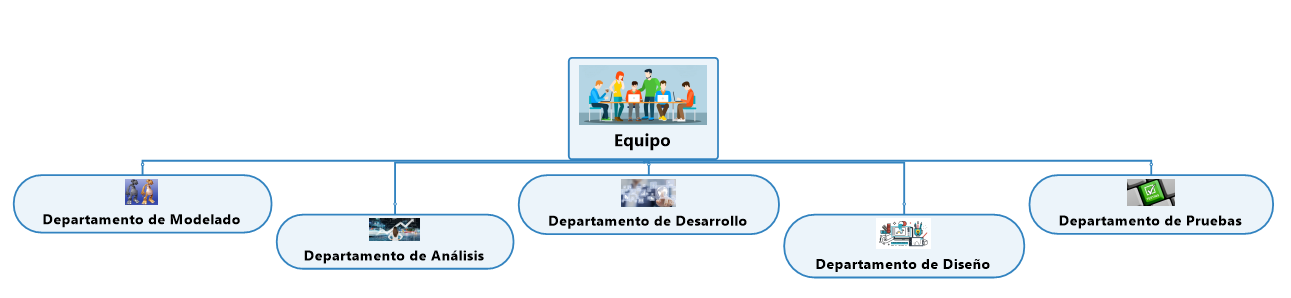
\includegraphics[scale=0.50]{imagenes/diagramaEstructura_2.png}
	\caption{\label{fig:diagramaEstructura}Diagrama estructura - Formulario OM2}
\end{figure}

\section{Formulario OM-3: Descomposición del Proceso de Negocio.}

Descripción del proceso de interés a partir de las tareas que lo componen.

\begin{table}[H]
  \centering
  \resizebox{18,0cm}{!}{
    \begin{tabular}{|c|c|c|c|c|c|c|}
      \hline
      \multicolumn{3}{|c}{\textbf{Modelo de Organización}} & \multicolumn{4}{|c|}{\textbf{Formulario OM-3: Descomposición de los Procesos}}\\
      \hline \hline
      \textsc{N\textordmasculine} & \textsc{Tarea} & \textsc{Realiza\-da por} & \textsc{¿Dónde?} & \textsc{Recursos de Conocimiento} & \textsc {¿In\-ten\-si\-va en Conocimiento?} & \textsc{Im\-por\-tan\-cia} \\
      \hline

      1 & Análisis de mercado & \multicolumn{1}{|p{6.0cm}|}{\centering Inversor (usuario)}& \multicolumn{1}{|p{5.0cm}|}{\centering En PC del inversor (usuario)} & \multicolumn{1}{|p{6.0cm}|}{\centering Experiencia en análisis de mercado de divisas.\\ Apoyo de herramientas de lectura de mercado} & Sí (elevado) & Alta \\
      \hline
      2 & Introducir datos gestión & \multicolumn{1}{|p{6.0cm}|}{\centering Inversor (usuario)} & \multicolumn{1}{|p{5.0cm}|}{\centering En el PC del inversor (usuario)} & \multicolumn{1}{|p{6.0cm}|}{\centering Experiencia por parte del inversor (usuario)} & Sí (moderado) & Alta \\
      \hline
      3 & Operación Comprar & \multicolumn{1}{|p{6.0cm}|}{\centering Inversor (usuario )}& \multicolumn{1}{|p{5.0cm}|}{\centering En PC del inversor (usuario)} & \multicolumn{1}{|p{6.0cm}|}{\centering Experiencia en compra de activos en mercado de divisas} & Sí (elevado) & Máxima \\
      \hline
      4 & Operación vender & \multicolumn{1}{|p{6.0cm}|}{\centering Inversor (usuario)}& \multicolumn{1}{|p{5.0cm}|}{\centering En PC del inversor (usuario)} & \multicolumn{1}{|p{6.0cm}|}{\centering Experiencia en venta de activos en mercado de divisas} & Sí (elevado) & Máxima \\
      \hline      
      5 & \multicolumn{1}{|p{6.0cm}|}{\centering Gestionar las operativas abiertas} & \multicolumn{1}{|p{6.0cm}|}{\centering Inversor (usuario)} &  \multicolumn{1}{|p{5.0cm}|}{\centering En PC del inversor (usuario)} & \multicolumn{1}{|p{6.0cm}|}{\centering Experiencia en gestiornar las operativas de compra y venta de activos al mercado de divisas} & Sí (elevado) & Máxima \\
      \hline
    \end{tabular}
  }
	\caption{\label{tab:OM3}Descomposición del proceso de negocio - OM3}
\end{table}

\section{Formulario OM-4: Activos de Conocimiento}
%%%%%%%%%%%%%%%%%%%%%%%%%%%%%%%%%%%%%%%%%%%%%%%%%%%%%%%%%%%%%%%%%%%%%%%%%%%%%%%

Descripción del componente \textit{conocimiento} del modelo de la organización.

\begin{table}[H]
  \centering
  \resizebox{17,5cm}{!}{
    \begin{tabular}{|c|c|c|c|c|c|c|}
      \hline
      \multicolumn{3}{|c}{\textbf{Modelo de Organización}} & \multicolumn{4}{|c|}{\textbf{Formulario OM-4: Activos de Conocimiento}}\\
      \hline \hline
      \textsc{Recurso de Conocimiento} & \textsc{Pertenece} & \textsc{Usado en} & \textsc{¿Forma Cor\-recta?} & \textsc{¿Lugar Cor\-recto?} & \textsc {¿Tiempo Cor\-recto?} & \textsc{¿Calidad Cor\-recta?} \\
      \hline
      \multicolumn{1}{|p{6.0cm}|}{\centering Experiencia en especulación de activos financieros} & \multicolumn{1}{|p{6.0cm}|}{\centering Expertos en especulación en mercados de activos} & \multicolumn{1}{|p{6.0cm}|}{\centering Tareas 3, 4 y 5 de OM-3} & \multicolumn{1}{|p{6.0cm}|}{\centering No, el conocimiento reside en el experto (inversor)} & - & - & \multicolumn{1}{|p{6.0cm}|}{\centering Sí, teniendo en cuenta que son aproximaciones (no se puede determinar siempre un resultado ganador)} \\
      \hline
    \end{tabular}
  }
	\caption{\label{tab:OM4}Activos de conocimiento - OM4}
\end{table}
 

\section{Formulario OM-5: Análisis de viabilidad}


Elementos a considerar en el análisis de la viabilidad del proyecto. Nota: para mayor comodidad, en este apartado se puede prescindir del formato ``tabla'' y transformarla en subsecciones (comando subsubsection) manteniendo los mismos epígrafes de la primera columna.

\begin{table}[H]
  \centering
  \resizebox{17.0cm}{!}{
    \begin{tabular}{|l|l|} 
      \hline
      \textbf{Modelo de Organización} & \textbf{Formulario OM-5: Elementos del Documento de Viabilidad}\\ 
      \hline\hline
      \textsc{Viabilidad Empresarial} & \multicolumn{1}{p{15.0cm}|}{Dado a que éste sería el segundo proyecto de nuestra empresa, disponemos de un historial que nos ayude a estimar los beneficios. Hemos aproximado un beneficio económico mínimo del 30\% del coste del capital invertido, así como experiencia y conocimiento en el ámbito empresarial. \newline 
      Al ser los socios aquellos que llevaremos a cabo el desarrollo de este proyecto, estimamos que el coste será de aproximadamente 4.000\euro/mes (teniendo en cuenta alquiler de instalaciones para llevar a cabo el trabajo, dietas, etc) durante un período de 6 meses, resultando en un total de 24.000\euro  aproximadamente. \newline
      Es un proyecto de alto riesgo para el capital inicial invertido en ese proyecto, puesto que no afectará el funcionamiento de la empresa, ya que la misma ya se encuentra operativa y recibiendo beneficios de un proyecto anterior con las mismas caractarísticas.}\\
      \hline
    \end{tabular}
  }
  \caption{\label{tab:OM5}Formulario OM-5 (Parte 1). Viabilidad Empresarial}
\end{table}

\begin{table}[H]
  \centering
  \resizebox{17.0cm}{!}{
    \begin{tabular}{|l|l|} 
      \hline
      \textbf{Modelo de Organización} & \textbf{Formulario OM-5: Elementos del Documento de Viabilidad}\\ 
      \hline\hline
      \textsc{Viabilidad Técnica} & \multicolumn{1}{p{15.0cm}|}{En la aplicación Especulador Experto, el proceso de especular en los mercados de divisas (Forex) tiene una complejidad elevada debido a que en el sistema tenemos una base de datos de los activos financieros de Forex muy extensa y tendría que estar conectada a tiempo real con las fluctuaciones de los precios de esos activos, lo que provoca que nuestro sistema tenga mucho conocimiento almacenado y varios procesos de razonamiento a realizar. En nuestra aplicación, el tiempo es un recurso crítico, debido a que en un pequeño margen temporal, los valores de los activos involucrados fluctuan y no se puede hacer nada al respecto. \newline
      La calidad de nuestro sistema está basada en los beneficios que podremos conseguir a la larga con nuestra aplicación: si la aplicación produce beneficios, entonces nuestro sistema es válido (siempre ha de comprobarse de manera exhaustiva). Al ser una aplicación desarrollada para pequeños inversores las interfaces tienen que ser lo más simples e intuitivas posibles.} \\
      \hline
    \end{tabular}
  }
  \caption{\label{tab:OM5-2}Formulario OM-5 (Parte 2). Viabilidad Técnica}
\end{table}

\begin{table}[H]
  \centering
  \resizebox{17.0cm}{!}{
    \begin{tabular}{|l|l|} 
      \hline
      \textbf{Modelo de Organización} & \textbf{Formulario OM-5: Elementos del Documento de Viabilidad}\\ 
      \hline\hline
      \textsc{Viabilidad del Proyecto} & \multicolumn{1}{p{15.0cm}|}{El personal tiene el compromiso de llevar a cabo los pasos necesarios para la realización del proyecto, estando así disponibles los recursos necesarios para su realización, ya sea tiempo, presupuesto, equipamiento o el ya mencionado personal, los cuales parten con el conocimiento y capacidades necesarias.\newline
      Las expectativas son realistas, dentro de un marco optimista, para un proyecto novedoso que se incorpora al mercado, el cual busca obtener los mejores resultados posibles. Para lograr todo lo anterior se cuenta con una buena organización y comunicación tanto interna como externa en el proyecto.\newline
      Por último, como ya se ha dicho, al ser un proyecto novedoso, existe la posibilidad de que la aplicación no vaya a tener los mismos éxitos de comercialización que la aplicación anterior desarrollada, pero como se trata de expandir un nuevo mercado y la experiencia de un proyecto similar, creyemos que nos valdrá el esfuerzo en todos los sentidos.} \\
      \hline
    \end{tabular}
  }
  \caption{\label{tab:OM5-3}Formulario OM-5 (Parte 3). Viabilidad del Proyecto}
\end{table}

\begin{table}[H]
  \centering
  \resizebox{17.0cm}{!}{
    \begin{tabular}{|l|l|} 
      \hline
      \textbf{Modelo de Organización} & \textbf{Formulario OM-5: Elementos del Documento de Viabilidad}\\ 
      \hline\hline
      \textsc{Acciones propuestas} & \multicolumn{1}{p{15.0cm}|}{Después del análisis realizado, se ha concluido que se llevará el proyecto adelante, incluyendo éste todas las tareas especificadas en el OM-3 correspondientes al proceso de "Especulación en Mercado de Divisas". \newline
        Los resultados esperados son una mejor gestion del tiempo, para asegurar el mismo beneficio que necesitaba de una persona pendiente del mercado ahorrandonos los nervios y ganando una toma de decisiones mas veloz.\newline
      Las acciones requeridas serian diseñar un motor de inferencia para sustituir al usuario experto para que tome decisiones de forma totalmente autonoma con una minima entrada de datos que serian el riesgo que estamos dispuestos a asumir y el numero maximo de operativas simultaneas a realizar.\newline
      Los riesgos son no solo no lograr el beneficio esperado ya que el sistema estaria diseñado para no tener mas perdidas de las asumidas por el usuario.} \\
      \hline
    \end{tabular}
  }
  \caption{\label{tab:OM5-4}Formulario OM-5 (Parte 4). Acciones Propuestas}
\end{table}